

\subsection{Traditional Distance Metrics}


\label{simple}

\subsubsection{Minkowski Distance}
The Minkowski distance of order $p$ (where $p$ is an integer) between two points $\mathbf{x}=\{x_1,x_2,\dots,x_n\}$ and $\mathbf{y}=\{y_1,y_2,\dots,y_n\}$ is defined as
$$d(\mathbf{x},\mathbf{y})=\left( \sum_{i=1}^n |x_i-y_i|^p\right)^{\frac{1}{p}}$$
When order $p$ in Minkowski distance varies, we can get different distance metrics.

\paragraph{Manhattan Distance}
When $p$ equals 1, we get Manhattan distance as
$$d(\mathbf{x},\mathbf{y})=\sum_{i=1}^n |x_i-y_i|$$

\paragraph{Euclidean Distance}
When $p$ equals 2, we have Euclidean distance as
$$d(\mathbf{x},\mathbf{y})=\sqrt{\sum_{i=1}^n (x_i-y_i)^2}$$
Euclidean distance is the most commonly used distance metric and it is the default metric in KNN of \texttt{sklearn}.

\paragraph{Chebyshev Distance}
In the limiting case of $p$ reaching infinity, we obtain the Chebyshev distance:
$$d(\mathbf{x},\mathbf{y})=\max_i |x_i-y_i|$$

\subsubsection{Cosine Distance}
Cosine similarity measures the similarity between two vectors of an inner product space. It is measured by the cosine of the angle between two vectors and determines whether two vectors are pointing in roughly the same direction.
$$\cos(\mathbf{x},\mathbf{y})=\frac{\mathbf{x}^T\mathbf{y}}{\|\mathbf{x}\|\|\mathbf{y}\|}$$

The resulting similarity ranges from $-1$ meaning exactly opposite, to 1 meaning exactly the same, with 0 indicating orthogonality or decorrelation. Therefore, the cosine distance is defined as,
$$d(\mathbf{x},\mathbf{y})=1-\cos(\mathbf{x},\mathbf{y})$$

When $\mathbf{x}$ and $\mathbf{y}$ are normalized to unit length, $\|\mathbf{x}\|=\|\mathbf{y}\|=1$, the relationship between Euclidean distance and cosine similarity is
$$d_{euc}(\mathbf{x},\mathbf{y})=\sqrt{2-2\cos(\mathbf{x},\mathbf{y})}$$



\subsection{Supervised Metric Learning}
% http://contrib.scikit-learn.org/metric-learn/supervised.html
\label{supervised}
    As the name suggests, Supervised Metric Learning takes each point x and its label y as an input, then it trys to learn a distance to make the samples in the same class have a relatively close measure while the samples in different classes have a far away distance with others. We show an intuitive example of metric learning in Figure \ref{fig:ml}. Commonly we project samples into the learned metric space and use several neighbors of samples as distance measure. Besides, sometimes the sample features are first reduced in dimension. In this section, we will use four supervised metric learning methods: LMNN, NCA, LFDA and MLKR.
    
    \begin{figure}[htbp]
        \centering
        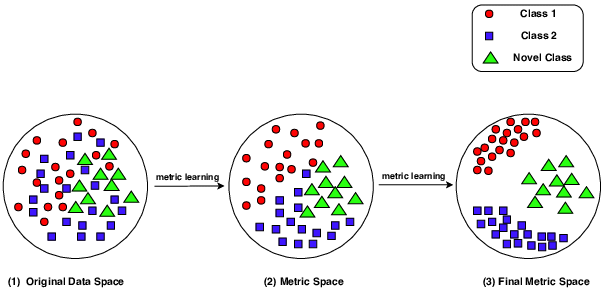
\includegraphics[width=0.7\linewidth]{img/metric-learning.png}
        \caption{An Intuitive Example of Metric Learning}
        \label{fig:ml}
    \end{figure}

\subsubsection{LMNN: Large Margin Nearest Neighbor Metric Learning}

    Large Margin Nearest Neighbor(LMNN)\cite{LMNN} classification is a supervised metric learning method based on sem-idefinite programming. This algorithm can be regarded as an optimization of KNN algorithm using Mahalanobis distance to some extent. 
    
    % As is well known, KNN takes some samples that has been classified in advance, then it calculates the distance between test sample and all trainning samples to select the k nearest samples to vote.
    As is well known, KNN usually takes simple distance metrics as its distance measure such as euclidean distance, manhattan distance. However, this makes all features weighted equally. To improve on that, LMNN tries to learn a Mahalanobis distance metric in the KNN classification setting.
    
     Suppose we have a distance metric methods:
     $$
        D_{\mathbf{L}}(x_i, x_j) = \|\mathbf{L}(x_i, x_j)\|_2^2
     $$
    when $\mathbf{M} = \mathbf{L}^T \mathbf{L}$, the Mahalanobis distance is defined as follow:
    $$
        D_{\mathbf{M}}(x_i, x_j) = (x_i - x_j)^T \mathbf{M} (x_i - x_j)
    $$
    Then the goal of distance measurement learning can be expressed in two aspects:
    (1) learn a linear transformation: $ \vec{x}' = \mathbf{L} \vec{x}$ (2) learn $\mathbf{M} = \mathbf{L}^T \mathbf{L}$. It is possible for some types of distance measures to learn convex optimizations on a cone represented by a positive semi-definite matrix $\mathbf{M}$.
    
    For LMNN, there are two aspects we should focus on: (1) Each training input $\vec{x}_i$ should have the same label $y_i$ as its k nearest neighbor samples. (2) If sample $\vec{x}_i$ and $\vec{x}_j$ with different labels should be widely separated during training.
    We define two loss function: $\varepsilon_{\text{pull}}$ corresponds to samples with same labels while $\varepsilon_{\text{push}}$ corresponds to the opposite:
    $$
    \begin{aligned}
       \varepsilon_{\text {pull }}(\mathbf{L}) &= \sum_{j \rightsquigarrow i}\left\|\mathbf{L}\left(\vec{x}_{i}-\vec{x}_{j}\right)\right\|^{2} \\
       \varepsilon_{\text {push }}(\mathbf{L}) &= \sum_{i, j \rightsquigarrow i} \sum_{l}\left(1-y_{i l}\right)\left[1+\left\|\mathbf{L}\left(\vec{x}_{i}-\vec{x}_{j}\right)\right\|^{2}-\left\|\mathbf{L}\left(\vec{x}_{i}-\vec{x}_{l}\right)\right\|^{2}\right]_{+}
    \end{aligned}
    $$
    merge two loss function, we get:
    $$
        \varepsilon(\mathbf{L}) = (1-\mu) \varepsilon_{\text {pull }}(\mathbf{L})+\mu \varepsilon_{\text {push }}(\mathbf{L})
    $$
    
    So the Object function is:
    $$
        \min \sum_{i, j} \mu_{ij} \| \mathbf{L}(\vec{x}_i - \vec{x}_j) \|^2 + c \sum_{i,j,l} \mu_{ij}(1 - y_{ij})\left [ 1 + \| \mathbf{L}(\vec{x}_i - \vec{x}_j) \|^2 - \| \mathbf{L}(\vec{x}_i - \vec{x}_l) \|^2 \right]_{+}
    $$
    An example of LMNN algorithm is shown in Figure \ref{fig:lmnn}:
    \begin{figure}[htbp]
        \centering
        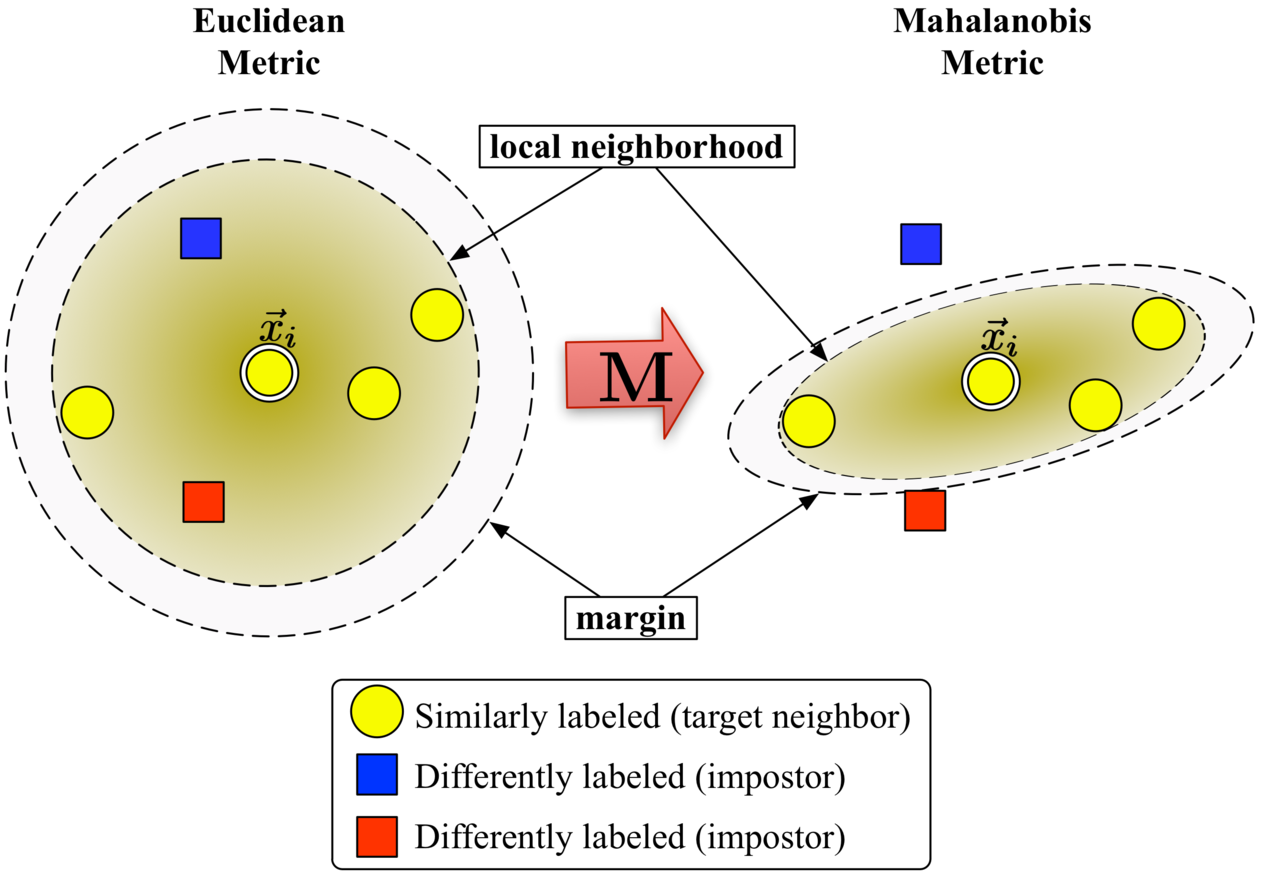
\includegraphics[width=0.6\linewidth]{img/Lmnn-principle.png}
        \caption{An Intuitive Example of LMNN Algorithm}
        \label{fig:lmnn}
    \end{figure}
    

        
\subsubsection{NCA: Neighborhood Components Analysis}


        Neighbourhood components analysis(NCA)\cite{NCA} algorithm is another supervised metric learning algorithm. The goal of NCA is similar as LMNN, it aims to classify input samples in different classes according to a learning metric distance. It find a linear transform of input samples to maximize the leave-one-out(LOO) classification performance.
        
        We have showed that the  Mahalanobis distance can be defined as: $D_{\mathbf{M}}(x_i, x_j) = (x_i - x_j)^T \mathbf{M} (x_i - x_j)$, where $\mathbf{M}$ is a  positive semi-definite matrix and can be expressed as $\mathbf{M} = \mathbf{L}^T \mathbf{L}$. We define an objective function $f(\cdot)$ to describe classification accuracy in the transformed space. Then the objective function:
        $$
            \mathbf{L}^* = \arg \max_{\mathbf{L}} f(\mathbf{L})
        $$
        The we need to make $f(\cdot)$ to be differential, so we define:
        $$
            f(\mathbf{L}) = \sum_i \sum_{j \in C_i} p_{ij} = \sum_i p_i
        $$
        where
        $$
            p_{i j}=\left\{
            \begin{array}{ll} 
                \frac{e^{-\left\|\mathbf{L} x_{i} - \mathbf{L} x_{j}\right\|^{2}}}{\sum_{k} e^{-\left\|\mathbf{L} x_{i}-\mathbf{L} x_{k}\right\|^{2}}}, & \text {if} \quad j \neq i \\
                0, & \text {if} \quad j=i
            \end{array}\right.
        $$
        $p_{ij}$ is the probability of classifying neighbor j of point i, $C_i$ is a data points set with same class as i. Then $f(\mathbf{L})$ can be differential to find the optimal solution.
        % \begin{aligned}
        %         \frac{e^{-\| Ax_i - Ax_j\|^2}}{\sum_k e^{-\| Ax_i - Ax_k\|^2}} \text{if} j \neq i \\
        %         0   \text{if} j = i
        %         \end{aligned}
        % classifying sample data to different classses according to the given distance metric. 
    
        
\subsubsection{LFDA: Local Fisher Discriminant Analysis}
    
        Local Fisher Discriminant Analysis(LFDA)\cite{LFDA} algorithm is a combination of Linear Discriminant Analysis(LDA) and Locality-Preserving Projection(LPP), where LDA aims at maximize the distance of data between classes and minimize the distance within classes and LPP can keeps nearby data pairs also be closed in the embedding space. So LFDA has good performance in dealing with multi-modality for it preserves original data structure.
        
        LDFA defines matrix distances in pairs which is similar to LDA: the Fisher local scatter matrix within class is
        $$
            \mathbf{S}^{(w)} =\frac{1}{2} \sum_{i, j=1}^{n} W_{i j}^{(w)}\left(\mathbf{x}_{i}-\mathbf{x}_{j}\right)\left(\mathbf{x}_{i}-\mathbf{x}_{j}\right)^{T}
        $$
        and between class is:
        $$
            \mathbf{S}^{(b)} =\frac{1}{2} \sum_{i, j=1}^{n} W_{i j}^{(b)}\left(\mathbf{x}_{i}-\mathbf{x}_{j}\right)\left(\mathbf{x}_{i}-\mathbf{x}_{j}\right)^{T}
        $$
        where
        $$
            W_{i j}^{(w)}=\left\{
            \begin{array}{ll}
                0 \quad  & y_{i} \neq y_{j} \\
                \mathbf{A}_{i, j} / n_{l} \quad  & y_{i}=y_{j}
            \end{array}\right.
        $$
        $$
            W_{i j}^{(b)}=\left\{
            \begin{array}{ll}
                1 / n & y_{i} \neq y_{j} \\
                \mathbf{A}_{i, j}\left(1 / n-1 / n_{l}\right) & y_{i}=y_{j}
            \end{array}\right.
        $$
        $n$ denotes the total number of samples and $n_l$ denotes the number of samples in class $l$.
        
        The object function of LFDA is defined as:
        $$
            \mathbf{L}_{L F D A}=\arg \max _{\mathbf{L}}\left[\operatorname{tr}\left(\left(\mathbf{L}^{T} \mathbf{S}^{(w)} \mathbf{L}\right)^{-1} \mathbf{L}^{T} \mathbf{S}^{(b)} \mathbf{L}\right)\right]
        $$
        An example of LFDA algorithm is shown in Figure \ref{fig:lfda}:
        \begin{figure}[htbp]
            \centering
            \includegraphics[width=0.6\linewidth]{img/Lfda-principle.png}
            \caption{An Intuitive Example of LMNN Algorithm}
            \label{fig:lfda}
        \end{figure}
    

\subsubsection{MLKR: Metric Learning for Kernel Regression}
    
    
         Metric Learning for Kernel Regression(MLKR)\cite{MLKR} algorithm proposed a new strategy based on kernel regression, which can be applied with many types of kernel functions and distance metrics. It learns a distance function by minimizing the error of leave-one-out regression.
         
         The loss function is defined as
         $$
            \mathcal{L} = \sum_i (y_i - \hat{y_i})^2
         $$
         where $\hat{y_i}$ is a sample prediction get from kernel regression:
         $$
            \hat{y_i} = \frac{\sum_{j \neq i} y_i k_{ij}}{\sum_{j \neq i} k_{ij}}
         $$
         $k_{ij}$ is the weight defined as
         $$
            k_{ij} = \frac{1}{\sqrt{2 \pi} \sigma} \exp \left ( -\frac{d(\mathbf{x}_i, \mathbf{x}_j)}{\sigma^2}\right)
         $$
         where $d(\cdot, \cdot)$ is Mahalanobis distance. $d(\mathbf{x}_i, \mathbf{x}_j) = \| \mathbf{L} (\mathbf{x}_i - \mathbf{x}_j)  \|$.



\subsection{Weakly Supervised Metric Learning}

\label{weaksupervised}
There are also a group of metric learning methods based on pairs or triples of similar and dissimilar points. Since they pose fewer demands on the training data-set, we will refer to them as \emph{Weakly Supervised Metric Learning} methods. In this paper, we study four weakly supervised metric learning methods, namely ITML, LSML, SCML and RCA.




\subsubsection{ITML: Information Theoretic Metric Learning}

ITML\cite{ITML} minimizes the (differential) relative entropy (Kullback-Leibler divergence), between two multivariate Gaussians subject to constraints on the associated Mahalanobis distance, which can be formulated into a Bregman optimization problem by minimizing the LogDet divergence subject to linear constraints. This algorithm can handle a wide variety of constraints and can optionally incorporate a prior on the distance function. Unlike some other methods, ITML does not rely on an eigenvalue computation or semi-definite programming.

Given a Mahalanobis distance parameterized by $M$, its corresponding multivariate Gaussian is denoted as:
$$
p(\mathbf{x} ; \mathbf{M})=\frac{1}{Z} \exp \left(-\frac{1}{2} d_{\mathbf{M}}(\mathbf{x}, \mu)\right)=\frac{1}{Z} \exp \left(-\frac{1}{2}\left((\mathbf{x}-\mu)^{T} \mathbf{M}(\mathbf{x}-\mu)\right)\right)
$$
where $Z$ is the normalization constant, the inverse of Mahalanobis matrix $\mathbf{M}^{-1}$ is the covariance of
the Gaussian.


The ITML method is based on truth of similar/dissimilar pairs, which we will sample from the labeled groups. Given pairs of similar points $S$ and pairs of dissimilar points $D$, the distance metric learning problem is to minimize the LogDet divergence, which is equivalent as minimizing $\mathbf{K} \mathbf{L}\left(p\left(\mathbf{x} ; \mathbf{M}_{0}\right) \| p(\mathbf{x} ; \mathbf{M})\right)$
$$
\begin{array}{rl}
\min _{\mathbf{A}} D_{\ell \mathrm{d}}\left(M, M_{0}\right)& =\operatorname{tr}(\left.M M_{0}^{-1}\right)-\log \operatorname{det}\left(M M_{0}^{-1}\right)-n \\
\text { subject to } &d_{\mathbf{M}}\left(\mathbf{x}_{i}, \mathbf{x}_{j}\right) \leq u \quad \left(\mathbf{x}_{i}, \mathbf{x}_{j}\right) \in S \\
& d_{\mathbf{M}}\left(\mathbf{x}_{i}, \mathbf{x}_{j}\right) \geq l \quad \left(\mathbf{x}_{i}, \mathbf{x}_{j}\right) \in D
\end{array}
$$
where $u$ and $l$ is the upper and the lower bound of distance for similar and dissimilar pairs respectively, and $\mathbf{M}_{0}$ is the prior distance metric, set to identity matrix by default, $D_{\ell \mathrm{d}}(\cdot, \cdot)$ is the log determinant.

 
\subsubsection{LSML: Least Squared-residual Metric Learning}

LSML\cite{LSML} proposes a loss function for metric learning based on the relative distance comparison results of pairs. The loss function of each constraint $d\left(\mathbf{x}_{i}, \mathbf{x}_{j}\right)<d\left(\mathbf{x}_{k}, \mathbf{x}_{l}\right)$ is denoted as:
$$
\boldsymbol{H}\left(d_{\mathbf{M}}\left(\mathbf{x}_{i}, \mathbf{x}_{j}\right)-d_{\mathbf{M}}\left(\mathbf{x}_{k}, \mathbf{x}_{l}\right)\right)
$$
where $H(\cdot)$ is the squared Hinge loss function defined as:
$$
H(x)=\left\{\begin{array}{ll}
0 & x \leq 0 \\
x^{2} & x>0
\end{array}\right.
$$
The summed loss function $L(C)$ is the simple sum over all constraints $\boldsymbol{C}=\left\{\left(\mathbf{x}_{i}, \mathbf{x}_{j}, \mathbf{x}_{k}, \mathbf{x}_{l}\right): d\left(\mathbf{x}_{i}, \mathbf{x}_{j}\right)<d\left(\mathbf{x}_{k}, \mathbf{x}_{l}\right)\right\} .$ 

The distance metric learning problem becomes minimizing the summed loss function of all constraints plus a regularization term w.r.t. the prior knowledge:

$$
\min _{\mathbf{M}}\left(D_{l d}\left(\mathbf{M}, \mathbf{M}_{\mathbf{0}}\right)+\sum_{\left(\mathbf{x}_{i}, \mathbf{x}_{j}, \mathbf{x}_{k}, \mathbf{x}_{l}\right) \in C} H\left(d_{\mathbf{M}}\left(\mathbf{x}_{i}, \mathbf{x}_{j}\right)-d_{\mathbf{M}}\left(\mathbf{x}_{k}, \mathbf{x}_{l}\right)\right)\right)
$$

where $\mathbf{M}_{0}$ is the prior metric matrix, set as identity by default, $D_{l d}(\cdot, \cdot)$ is the LogDet divergence:

$$
\boldsymbol{D}_{l d}\left(\mathbf{M}, \mathbf{M}_{\mathbf{0}}\right)=\operatorname{tr}\left(\mathbf{M M}_{\mathbf{0}}\right)-\log \operatorname{let}(\mathbf{M})
$$

The minimizing goal is a convex objective function corresponding to the sum of squared residuals of constraints. The algorithm is considered as a simple, yet effective, algorithm since its sparsity extension leads to more stable estimation when the dimension is high and only a small amount of constraints is given.








\subsubsection{SCML: Sparse Compositional Metric Learning}

Some weakly supervised metric learning are based on \emph{triplet} samples. The semantic of a triplet of data-point is that the first point should be closer to the second point than to the third one.

SCML\cite{SCML} learns a squared Mahalanobis distance from triplet constraints by optimizing sparse positive weights assigned to a set of $K$ rank-one PSD bases. This can be formulated as an optimization problem with only $K$ parameters, that can be solved with an efficient stochastic composite scheme.
The Mahalanobis matrix $M$ is built from a basis set $B=\left\{b_{i}\right\}_{i=\{1, \ldots, K\}}$ weighted by a $K$ dimensional vector $w=\left\{w_{i}\right\}_{i=\{1, \ldots, K\}}$ as:
$$
M=\sum_{i=1}^{K} w_{i} b_{i} b_{i}^{T}=B \cdot \operatorname{diag}(w) \cdot B^{T} \quad w_{i} \geq 0
$$
Learning $M$ in this form makes it PSD by design, as it is a nonnegative sum of PSD matrices. The basis set $B$ is fixed in advance and it is possible to construct it from the data. The optimization problem over $w$ is formulated as a classic margin-based hinge loss function involving the set $C$ of triplets. A regularization $\ell_{1}$ is added to yield a sparse combination. The formulation is the following:
$$
\min _{w \geq 0} \sum_{\left(x_{i}, x_{j}, x_{k}\right) \in C}\left[1+d_{w}\left(x_{i}, x_{j}\right)-d_{w}\left(x_{i}, x_{k}\right)\right]_{+}+\beta\|w\|_{1}
$$
where $[\cdot]_{+}$ is the hinge loss.




\subsubsection{RCA: Relative Components Analysis}

RCA\cite{RCA1,RCA2,RCA3} learns metrics by pairs. It will generate a full rank Mahalanobis distance metric based on a weighted sum of \emph{in-chunklets} covariance matrices. It applies a global linear transformation to assign large weights to relevant
dimensions and low weights to irrelevant dimensions. Those relevant dimensions are estimated using \emph{``chunklets''}, subsets of points that are known to belong to the same class.

We will sample \texttt{chunk\_size} training points for each \texttt{num\_chunks} chunklets, so that the algorithm is efficient by simply computing
$$
\mathbf{C}=\frac{1}{n} \sum_{j=1}^{k} \sum_{i=1}^{n_{j}}\left(\mathbf{x}_{j i}-\hat{\mathbf{m}}_{j}\right)\left(\mathbf{x}_{j i}-\hat{\mathbf{m}}_{j}\right)^{T}
$$
where chunklet $j$ consists of $\left\{\mathbf{x}_{j i}\right\}_{i=1}^{n_{j}}$ with a mean $\hat{m}_{j} .$ The inverse of $\mathbf{C}^{-1}$ is used as the Mahalanobis matrix.

